\subsection{Installazione ambiente di sviluppo integrato WebStorm}
Per installare l'ambiente di sviluppo integrato WebStorm visitare la pagina \url{https://www.jetbrains.com/webstorm/download/}. Qui è possibile trovare il download per MacOS, Windows e sistemi operativi basati su Linux/Unix.
\\
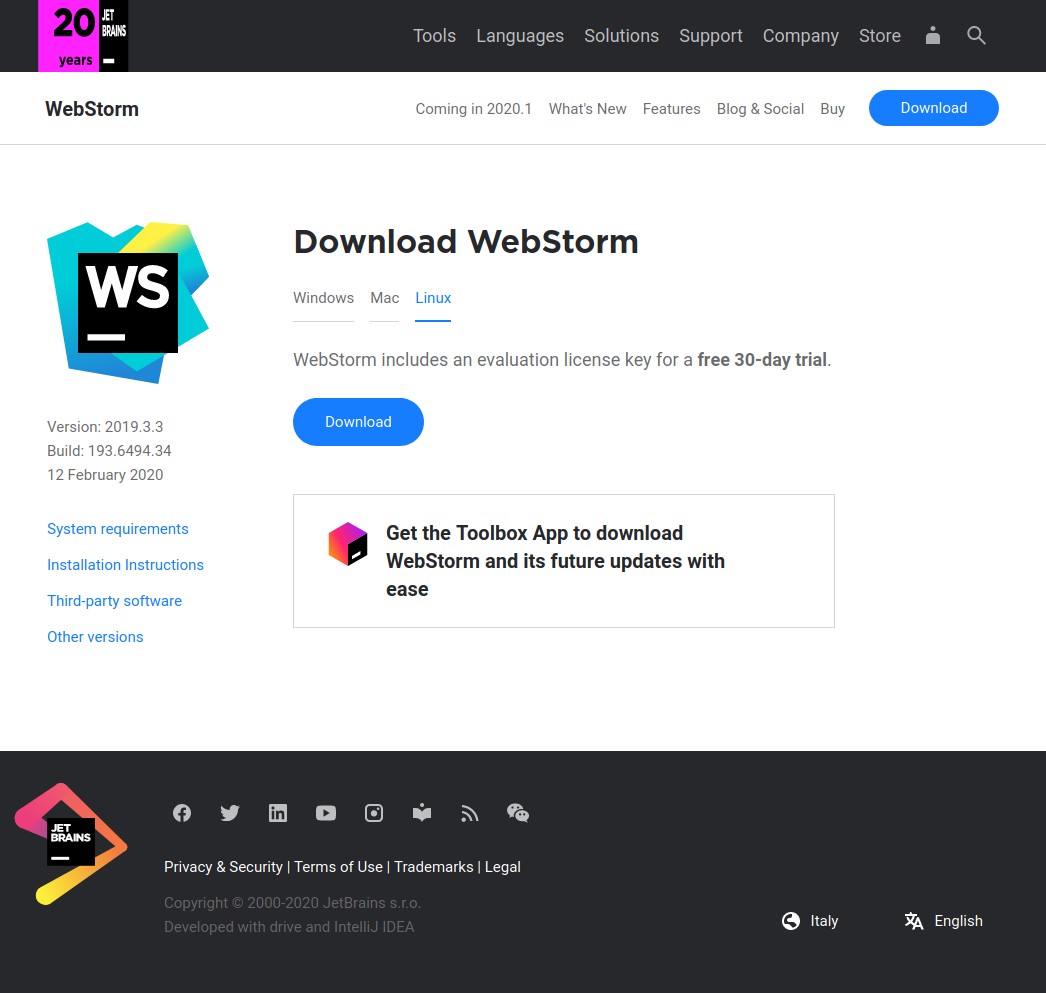
\includegraphics[width=\textwidth,height=\textheight,keepaspectratio]{img/webstorm.png}

\subsection{Installazione plugin SonarLint per WebStorm}
Per installare il plugin SonarLint per WebStorm aprire le impostazioni di WebStorm dal suo menù "File", Quindi nella sezione "Plugins" cercare ed installare "SonarLint".
\\
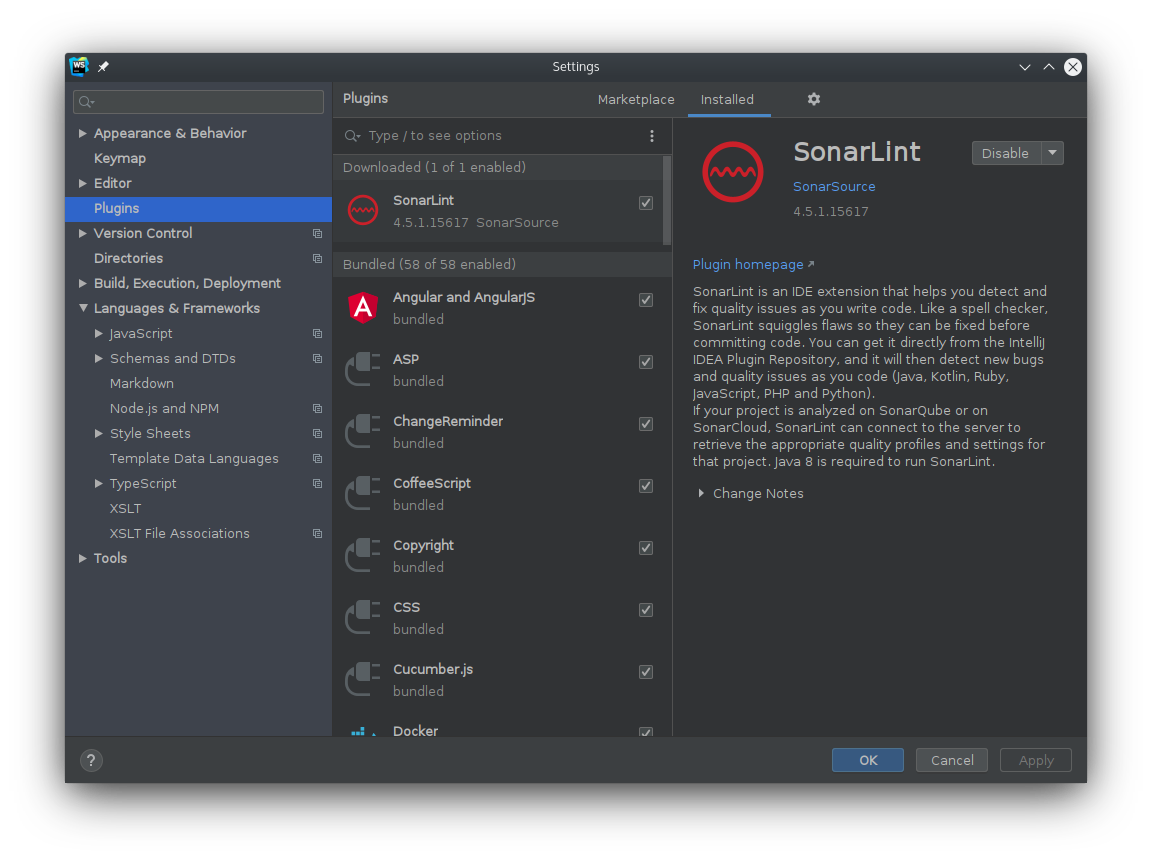
\includegraphics[width=\textwidth,height=\textheight,keepaspectratio]{img/sonarlint.png}

\subsection{Grafana}
Per installare Grafana\glosp visitare la pagina \url{https://grafana.com/get}. Qui è possibile trovare il download per MacOS, Windows e sistemi operativi basati su Linux/Unix.
\subsubsection{Eseguire il servizio WEB Grafana} Per eseguire il servizio WEB Grafana\glosp aprire la cartella "bin" dell'installazione grafana ed a seconda del sistema operativo eseguire:
\begin{itemize}
	\item \textbf{Windows}: fare doppio click sul file "grafana-server";
	\item \textbf{Linux, Mac}: eseguire in una shell 
		\begin{verbatim}
			./grafana-server web.
		\end{verbatim}
\end{itemize}
Collegarsi quindi con un browser all'indirizzo \url{http://localhost:3000/}; le credenziali richieste al primo avvio sono username "admin" e password "admin".
\\
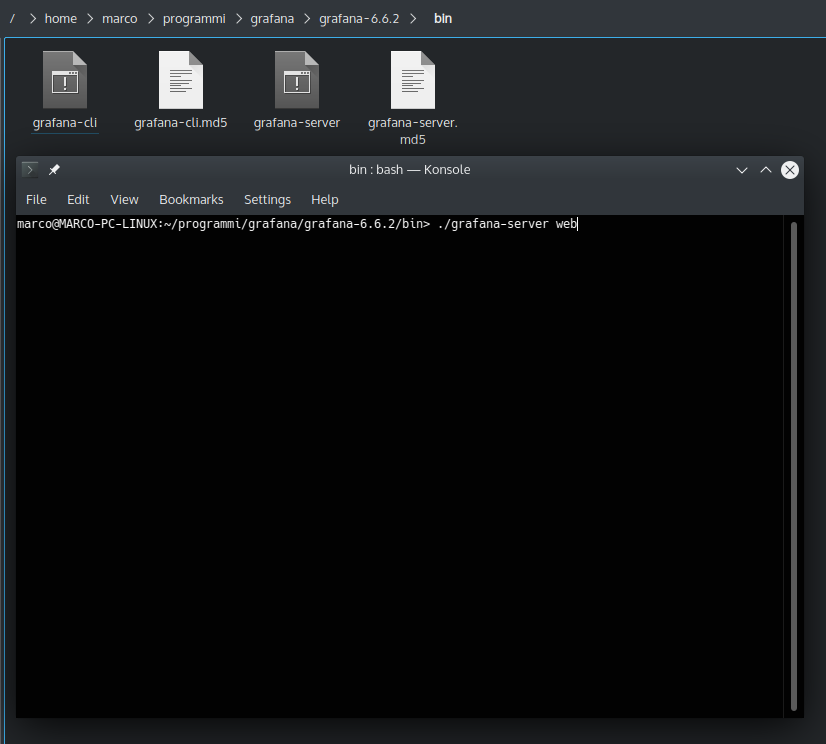
\includegraphics[width=\textwidth,height=\textheight,keepaspectratio]{img/grafana-server.png}

\subsection{Installazione plugin Grafana}
\subsubsection{Requisiti}
\begin{itemize}
	\item \textbf{Grafana\glo};
	\item \textbf{Node.js}: runtime Javascript che permette di eseguire codice Javascript fuori da un browser, l'installazione di npm (Node Package Manager) non è richiesta dato che viene installato automaticamente durante l'installazione di Node.js;
	\item \textbf{Git}: sistema di versionamento distribuito.
\end{itemize}

\subsubsection{Installazione degli strumenti}

\paragraph{Node}
Per installare il runtime Javascript Node.js si può visitare il sito \href{https://nodejs.org}. Qui è possibile trovare il download di Node.js per tutti i sistemi operativi. Alternativamente, su sistemi operativi basati su Linux è possibile utilizzare lo strumento di gestione di pacchetti fornito dal sistema operativo per installare i pacchetti del runtime Node.js. Di seguito un esempio:
\textbf{Debian/Ubuntu} \\
\begin{verbatim}
apt-get install nodejs
\end{verbatim}

\paragraph{Git}
Per installare il sistema di versionamento distribuito Git visitare la pagina \url{https://git-scm.com/downloads}. Qui è possibile trovare il download per MacOS, Windows e sistemi operativi basati su Linux/Unix.

\subsubsection{Installazione dell'applicazione}
\paragraph{Clonare la repository da GitHub}
Per clonare la repository dell'applicazione aprite un terminale e usate il comando cd per muovervi in una cartella del vostro computer, eseguite il comando: 
\begin{verbatim}git clone https://github.com/VRAM-Software/grafana_prediction.git
\end{verbatim}
Infine con il comando 
\begin{verbatim}
	cd ./grafana_prediction_plugin
\end{verbatim}
spostatevi nella cartella che contiene il codice sorgente del plugin.

\paragraph{Installare le dipendenze}
Per il corretto funzionamento dell'applicazione è necessario installare tutte le dipendenze elencate precedentemente, per farlo eseguite il comando npm install.

\paragraph{Eseguire il plugin}
Per eseguire l'applicazione è necessario copiare il contenuto del repository "grafana\_prediction\_plugin", ad eccezione delle cartelle "node\_modules" e "coverage", all'interno della cartella "data/plugins" dell'installazione Grafana\glo. Accedendo all'interfaccia web di Grafana\glosp si potrà quindi abilitare il plugin dall'apposita sezione plugins delle impostazioni di Grafana\glo.
\\
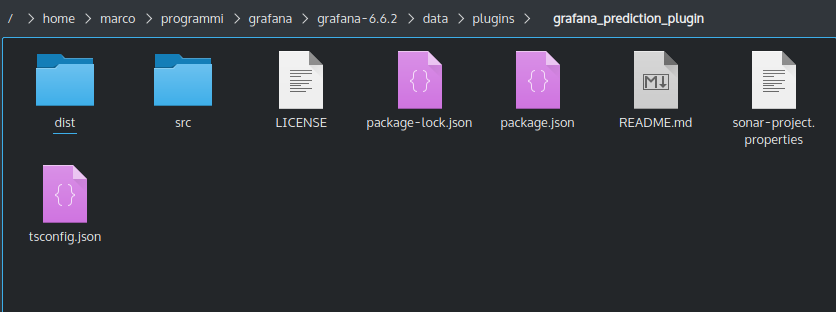
\includegraphics[width=\textwidth,height=\textheight,keepaspectratio]{img/plugin-directory.png}

\paragraph{Impacchettare il plugin}
Per generare una release di produzione basta eseguire il comando "npm run build" e successivamente creare un archivio zip dell'intero repository escludendo le cartelle "node\_modules" e "coverage". Questo plugin potrà poi essere distribuito per essere installato da altri utenti. 
